\documentclass{beamer}
\usepackage[utf8]{inputenc}
\usepackage{MnSymbol}
\usepackage{qtree}
\usepackage{amssymb}
\usepackage{extarrows}
\usepackage{tikz}
\usepackage{mathrsfs}
\usetikzlibrary{arrows,automata}
\usepackage{graphicx}
\usepackage{hyperref}
\usepackage{subcaption,graphicx}
\usetheme{CambridgeUS}  %% Themenwahl
\beamertemplatenavigationsymbolsempty
%\useoutertheme{split}
%\useinnertheme{rectangles}

%\usecolortheme{beaver}


\title{Bildbasierte Navigation mit Neuronalen Netzen: Kolloquium}
\author{Jan Robert Rösler}
\date{\today}

\begin{document}
\maketitle

\frame{\tableofcontents}

\section{Technischer Hintergrund}

\frame{\tableofcontents[currentsection]}

\begin{frame} 
  \frametitle{Deep Learning} 

\begin{figure}
	\centering
	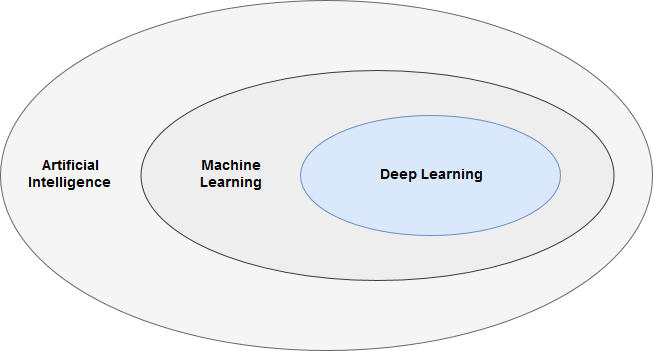
\includegraphics[width=.85\linewidth]{figures/Mengen.png}	 
	%\caption{}
	%Quelle: \protect\citeI{Architecture-ALVINN}
	\label{img:menge}
\end{figure}

\end{frame}


\begin{frame} 
\frametitle{Deep Learning} 
\centering
Künstliche neuronale Netze sind universelle Funktionsapproximatoren.\\

\begin{figure}
	\centering
	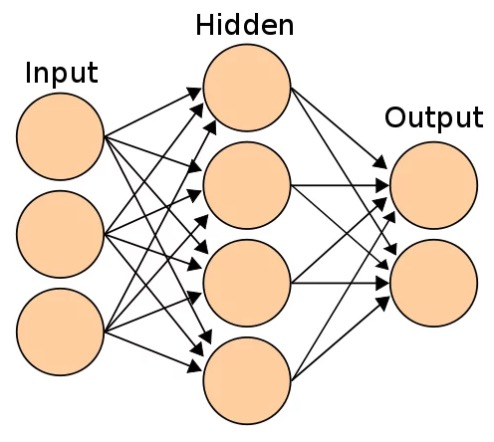
\includegraphics[width=0.4\linewidth]{figures/NN.jpg}
	%\quelle{https://cdn-images-1.medium.com/max/1600/1*q1M7LGiDTirwU-4LcFq7_Q.png}
	\label{img:nn}
\end{figure}

\end{frame}

\begin{frame} 
\frametitle{Deep Learning} 
\centering
Berechnung mit Backpropagation.\\

\begin{figure}
	\centering
	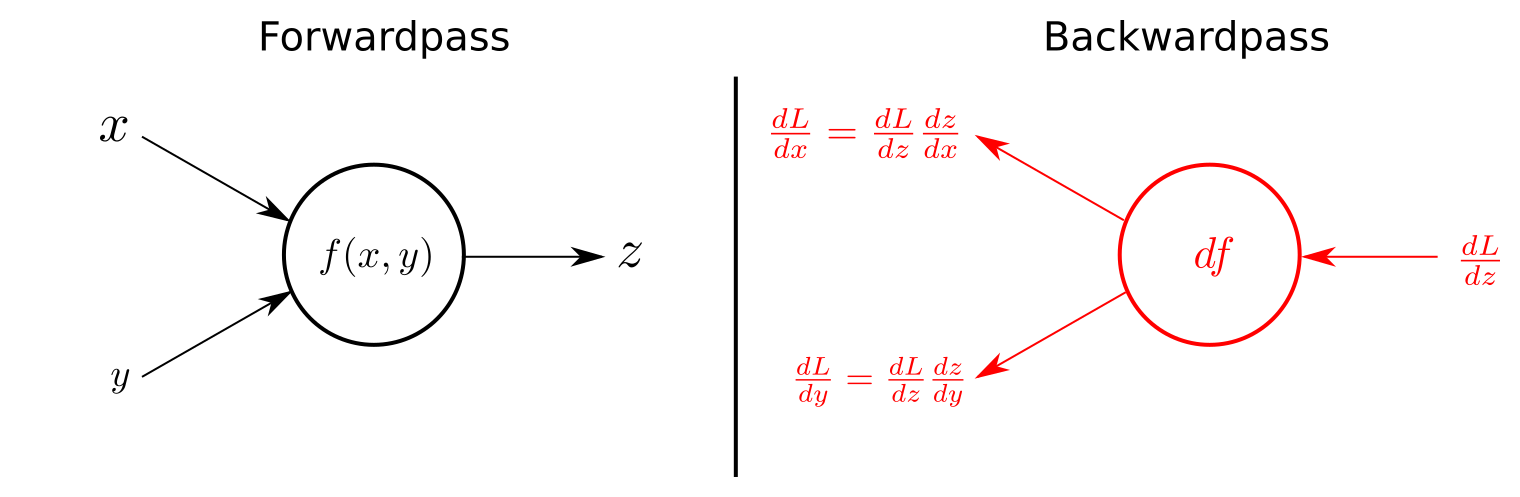
\includegraphics[width=\linewidth]{figures/chainrule.png}
	%\quelle{https://cdn-images-1.medium.com/max/1600/1*q1M7LGiDTirwU-4LcFq7_Q.png}
	\label{img:chainrule}
\end{figure}

\end{frame}




\begin{frame}

\frametitle{Deep Learning mit Bildern}
\framesubtitle{Wie können Bilder in neuronalen Netzen verarbeitet werden?}

\begin{columns}[T]

\begin{column}[T]{5cm}
Möglich:\\
Matrix zu einem einspaltigen Inputvektor umwandeln.\newline

\textcolor{red}{Problem:}
\begin{itemize}
\item{\textcolor{red}{Räumliche Information geht verloren}}
\item{\textcolor{red}{Hoher Rechenaufwand}}
\end{itemize}

\end{column}

\begin{column}[T]{5cm}
	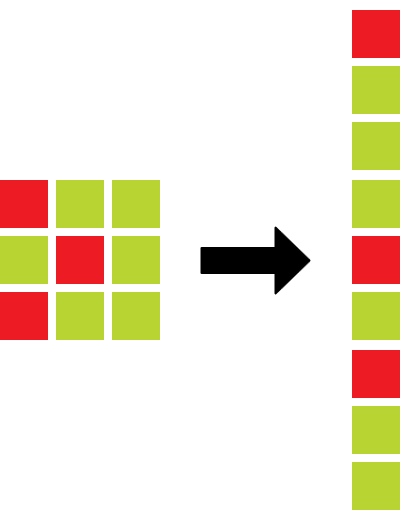
\includegraphics[scale=0.3]{figures/inputimage.png}	 
\end{column}

\end{columns}

\end{frame}


\begin{frame}
\frametitle{Convolutional Neural Network}
\framesubtitle{Convolutional-Layer}

\begin{columns}[T]

\begin{column}[T]{5cm}
\begin{itemize}
\item{Input Bilddaten als Matrix}
\item{Neuronenaktivität wird über diskrete Faltung mit Faltungsmatrix (convolution) berechnet}
\item{Extrahierung von Bildeigenschaften in feature-maps}
\end{itemize}


\end{column}

\begin{column}[T]{7cm}
	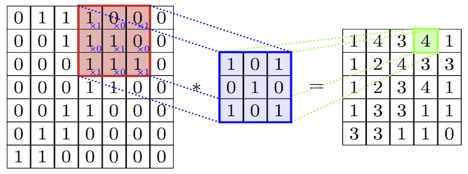
\includegraphics[scale=0.44]{figures/convolution.jpg}
	%Quelle: https://saama-dbe0.kxcdn.com/wp-content/uploads/2017/12/01.jpg?iv=136
\end{column}

\end{columns}

\end{frame}

\begin{frame}
\frametitle{Convolutional Neural Network}
\framesubtitle{Pooling-Layer}

Subsampling der prägnanten Bildteile.

\begin{figure}
	\centering
	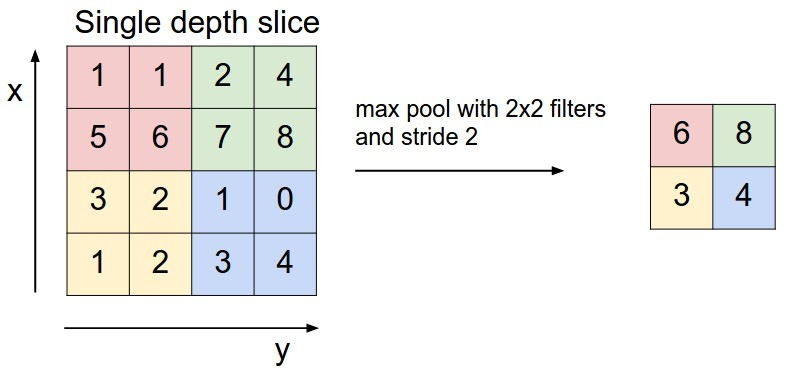
\includegraphics[width=\linewidth]{figures/maxpool.jpeg}
	%\quelle{http://cs231n.github.io/assets/cnn/maxpool.jpeg}
	\label{img:maxpooling}
\end{figure}
\end{frame}

\begin{frame}
\frametitle{Convolutional Neural Network}
\framesubtitle{Aktivierungsfunktion -  ReLU}
Das Rectified-Linear-Unit wandelt den mittels Faltung ermittelten Neuroneninput in den Output um. \textbf{F(x) = max(0,x)}

\begin{figure}
	\centering
	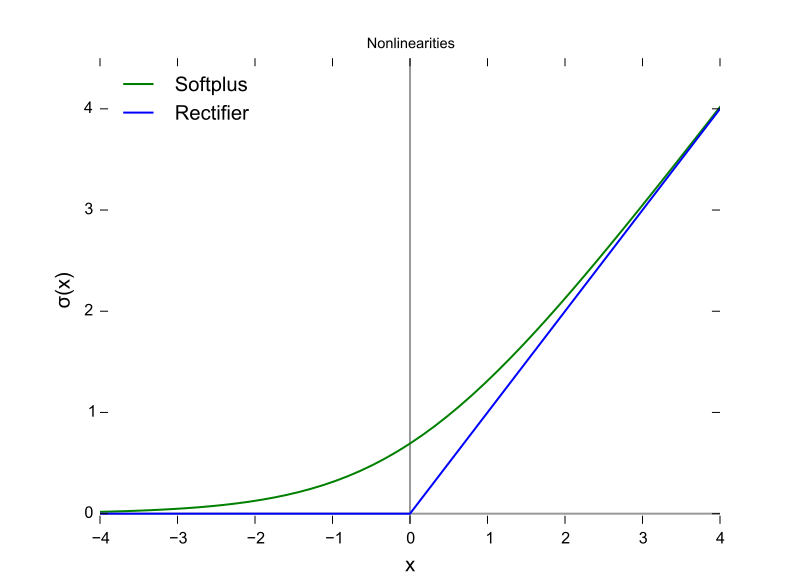
\includegraphics[width=0.7\linewidth]{figures/relu.png}
	%\quelle{https://en.wikipedia.org/wiki/Rectifier_(neural_networks)#/media/File:Rectifier_and_softplus_functions.svg}
	\label{img:relu}
\end{figure}
\end{frame}

\begin{frame}
\frametitle{Convolutional Neural Network}
\begin{figure}
	\centering
	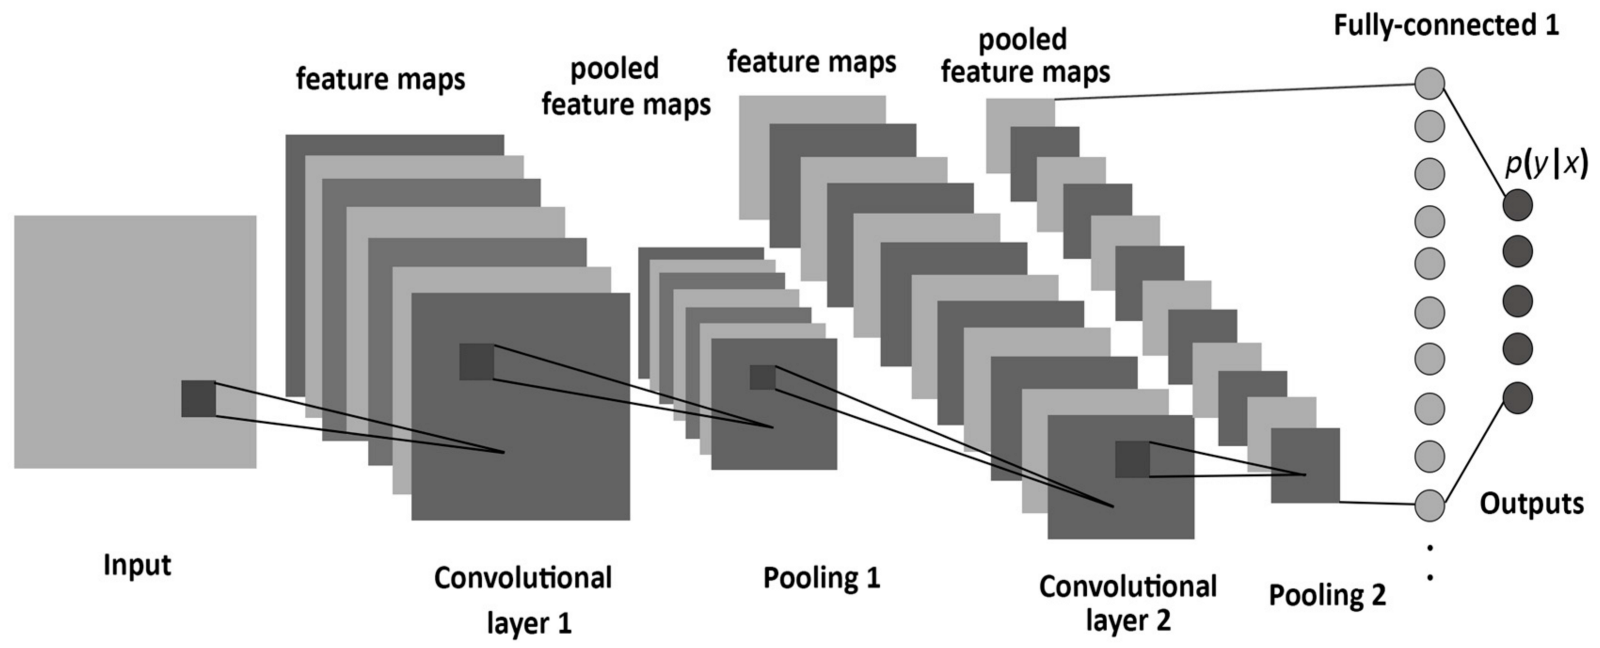
\includegraphics[width=\linewidth]{figures/network.png}
	%\quelle{https://cdn-images-1.medium.com/max/1600/1*dvDZzVJ88XWX-nLliWgvWw.png}
	\label{img:maxpooling}
\end{figure}

\end{frame}





\begin{frame}
\frametitle{Vanishing Gradient Problem}

Wird der durch Backpropagation berechnete Gradient an einer Stelle eines (tiefen) neuronalen Netzes sehr klein oder sogar Null, erfahren die Gewicht der früheren Layer sehr kleine oder gar keine Aktualisierungen mehr. Der ``verschwindende'' Gradient hält das Netz vom Lernen ab.
\end{frame}


\begin{frame}
\frametitle{Residual Networks}

\begin{columns}[T]

\begin{column}[T]{5cm}
\textbf{Annahme:}\\
Die Funktion $H(x)$ ist die optimale Lösung für ein Problem. Sie soll approximiert werden.

\end{column}

\begin{column}[T]{7cm}
	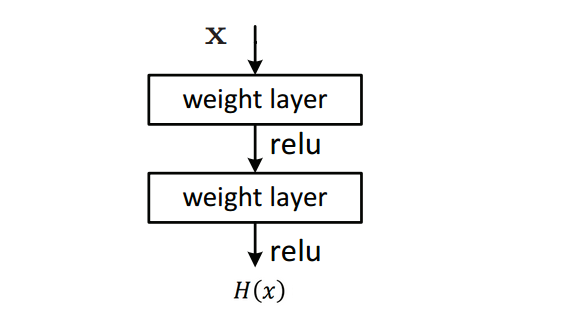
\includegraphics[scale=0.5]{figures/block.png}	 
\end{column}

\end{columns}
\end{frame}


\begin{frame}
\frametitle{Residual Networks}
\framesubtitle{Identity Shortcut}

\begin{columns}[T]

\begin{column}[T]{5cm}
\textbf{Umwandlung:}\\
Statt H(x) wird $H(x) = F(x) + x$ gelernt.\\ F(x) ist das Residual, die Differenz $H(x) - x$.


\end{column}

\begin{column}[T]{7cm}
	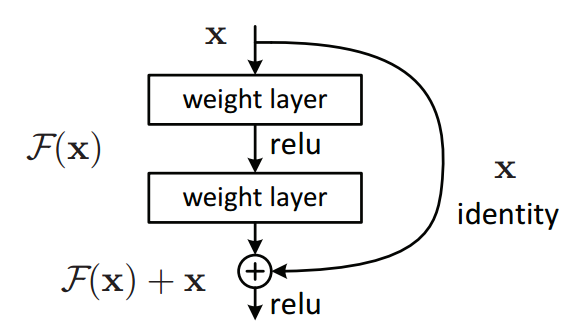
\includegraphics[scale=0.6]{figures/ResidualBlock.png}	 
\end{column}

\end{columns}
\end{frame}

\begin{frame}
\frametitle{Residual Networks}
\framesubtitle{Identity Shortcut}

\begin{columns}[T]

\begin{column}[T]{5cm}
\textbf{Vorteile:}\\
\begin{itemize}
\item{Freier Gradientenfluss}
\item{Durch lernen von F(x)=0 wird H(x) = x}\\
$\xrightarrow{}$Identitätsfunktion leicht zu erlernen
\end{itemize}


\end{column}

\begin{column}[T]{7cm}
	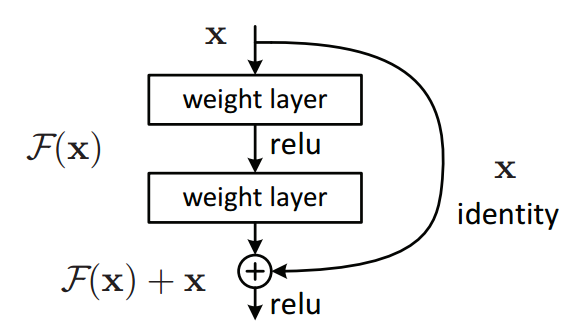
\includegraphics[scale=0.6]{figures/ResidualBlock.png}	 
\end{column}

\end{columns}
\end{frame}

\section{Idee}
\frame{\tableofcontents[currentsection]}

\begin{frame}
\frametitle{DroNet}
\textbf{Projekt der ETH Zürich:}\\
 Lenkwinkel- und Kollisionsbestimmung mit einem neuronalen Netz.\\
Trainiert auf einem öffentlichen Datensatz mit Fahrbahnbildern, angewendet auf einer Drohne.\\
\quad \\
\quad \\
\quad \\
\textbf{Input:}\\
200x200 Pixel Graustufenbild \\
\quad \\
\textbf{Output:}\\
Lenkwert von -1 (rechts) bis 1 (links) und Kollisionswahrscheinlichkeit in Prozent


\end{frame}

\begin{frame}
\frametitle{DroNet}
\framesubtitle{Architektur}
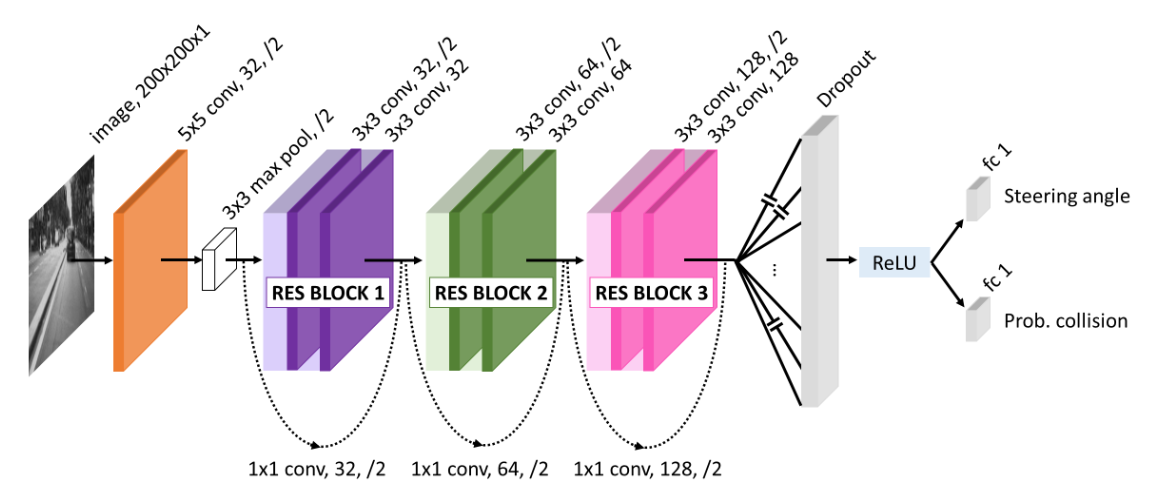
\includegraphics[width=\linewidth]{figures/Architecture-DRONET.png}	
\end{frame}


\begin{frame}
\frametitle{Idee}

\textbf{Anstoß:} DroNet Projekt ETH Zürich \\

\textbf{Rahmen:} Carolo-Cup\\

\textbf{Basis:} HAW Teststrecke, Carolo-Cup Fahrzeugplattform\\

\textbf{Ziel:} Entwicklung einer bildbasierten Fahrzeugsteuerung mit einem neuronalen Netz



\end{frame}


\section{Entwurf}
\frame{\tableofcontents[currentsection]}

\begin{frame}
\frametitle{Daten}
\framesubtitle{Bilder sammeln}

\begin{columns}[T]

\begin{column}[T]{5cm}
\begin{itemize}
\item{Algorithmus TeamWorstcase}
\item{ca 20.000 Aufnahmen}
\item{6000  davon geeignet für Training}

\end{itemize}

\end{column}

\begin{column}[T]{5cm}
	\begin{figure}
	\centering
	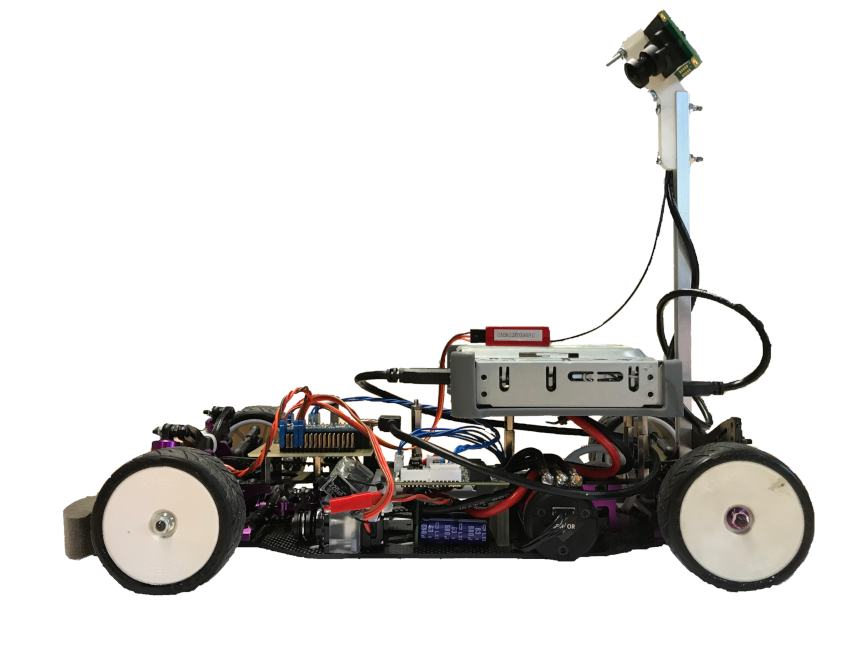
\includegraphics[width=0.4\linewidth]{figures/Fahrzeug.png}	 
	%\caption{}
	%Quelle: \protect\citeI{Architecture-ALVINN}
	\label{img:fahrzeug}
\end{figure}
\end{column}

\end{columns}




\end{frame}



\begin{frame}
\frametitle{Daten}
\framesubtitle{Bildverarbeitung}

\begin{minipage}{\textwidth}
\begin{figure}

	\begin{subfigure}{.25\textwidth}
		  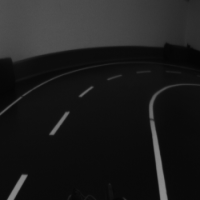
\includegraphics[scale=0.32]{figures/200x200.png}
	\end{subfigure}%
	\begin{subfigure}{.25\textwidth}
		  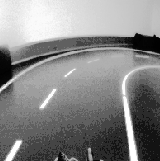
\includegraphics[scale=0.4]{figures/200x200Hist.png}
	\end{subfigure}%
	\begin{subfigure}{.25\textwidth}
		  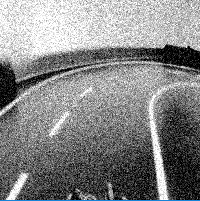
\includegraphics[scale=0.43]{figures/200x200Gauss.png}
	\end{subfigure}%
\end{figure}
\end{minipage}

\begin{minipage}{\textwidth}
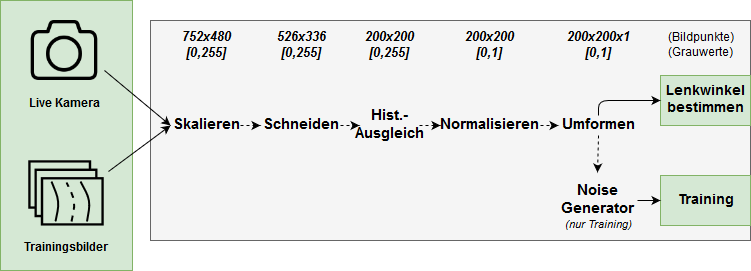
\includegraphics[width=\linewidth]{figures/Pipeline.png}	
\end{minipage}
\end{frame}

\begin{frame}
\frametitle{Architektur}
\framesubtitle{Anpassungen}
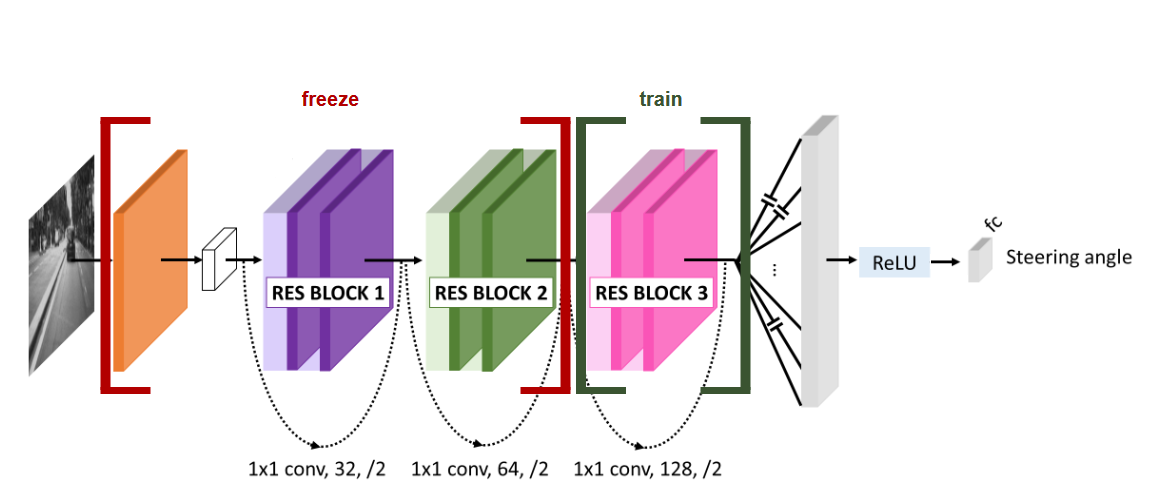
\includegraphics[width=\linewidth]{figures/Architecture-DRONET-FROZEN.png}	
\end{frame}

\begin{frame}
\frametitle{Training}
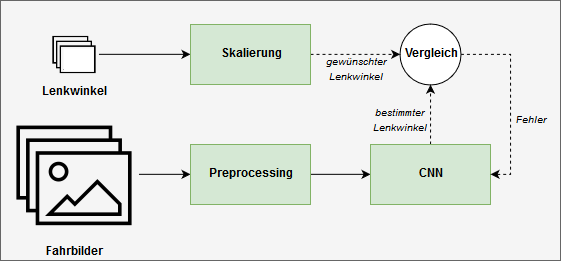
\includegraphics[width=\linewidth]{figures/Lernarchitektur.png}	 
\end{frame}

\begin{frame}
\frametitle{Steuerung}
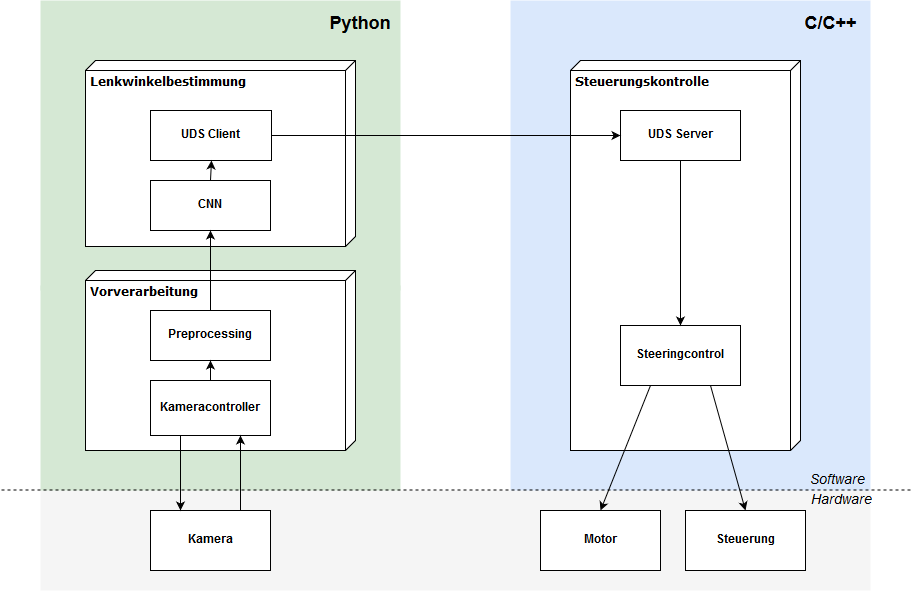
\includegraphics[width=\linewidth]{figures/Steuerung.png}	 

\end{frame}


\section{Ergebnis}
\frame{\tableofcontents[currentsection]}

\begin{frame}
\frametitle{Auswertung}
\framesubtitle{Training}

\begin{columns}[T]

\begin{column}[T]{5cm}
\begin{itemize}
\item{}


\end{itemize}


\end{column}

\begin{column}[T]{6cm}
	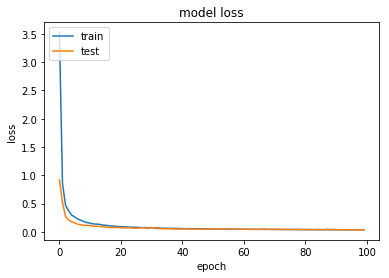
\includegraphics[scale=0.44]{figures/loss.png}
	%Quelle: https://saama-dbe0.kxcdn.com/wp-content/uploads/2017/12/01.jpg?iv=136
\end{column}

\end{columns}

\end{frame}


\begin{frame}
\frametitle{Auswertung}
\framesubtitle{Testfahrt}

\centering
{\huge $\xrightarrow{}$} {\huge Aufnahmen} 

\end{frame}

\begin{frame}
\frametitle{Testfahrt}
\framesubtitle{Performance messen - Metrik}
\begin{equation}
Autonomiewert = (1 -  \frac{\text{Anzahl Fehler}\cdot 2 s}{\text{Fahrzeit in Sekunden}})\cdot 100
\end{equation}
\end{frame}

\begin{frame}
\frametitle{Testfahrt}
\framesubtitle{Performancemessung}
\begin{table}[h]
  \begin{center}
    \label{tab:testfahrten}
    \begin{tabular}{l|c|r} 
      \textbf{Algorithmus} & \textbf{Fehler Runde 1} & \textbf{Fehler Runde 2}\\
      \hline
      DroNet & 16 & 12\\
      Carolo-Projekt & 7 & 11\\
       BA-RR& 3 & 5\\
    \end{tabular}
  \end{center}
\end{table}
Gesamtfahrzeit = 120 Sekunden\\
Runde 1 im Uhrzeigersinn (60 Sekunden)\\
Runde 2 gegen den Uhrzeigersinn (60 Sekunden)

\end{frame}

\begin{frame}
\frametitle{Testfahrt}
\framesubtitle{Performancevergleich}

\begin{table}[h]
  \begin{center}
    \label{tab:autonomie}
    \begin{tabular}{l|r}
      \textbf{Algorithmus} & \textbf{Autonomiewert} \\
      \hline
      DroNet & 53 \% \\
      Carolo-Projekt & 70 \%  \\
       BA-RR& 87 \% \\
    \end{tabular}
  \end{center}
\end{table}

\end{frame}

\begin{frame}
\frametitle{Auswertung}
\framesubtitle{Visualisierung}
Sichtbarmachen von wichtigen Bildbereichen:\\
Betrachtung der Veränderung des Outputs bei einer Veränderung des Inputs.\\
Hervorheben der Bildpunkte, die für\\
\begin{itemize}
\item{eine Erhöhung (Linkskurve)}
\item{eine Verminderung (Rechtskurve)}
\end{itemize}
des Lenkwerts besonders von Bedeutung sind.
Hellere Bildbereiche kennzeichnen diese Bedeutung.

\end{frame}


\begin{frame}
\frametitle{Attention-Heatmap}
\framesubtitle{Linkskurve}
\begin{figure}
	\centering
	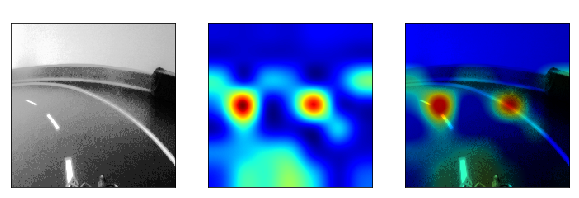
\includegraphics[width=\linewidth]{figures/left.png}	 
	%\caption{}
	%Quelle: \protect\citeI{Architecture-ALVINN}
	\label{img:left}
	\end{figure}
\end{frame}

\begin{frame}
\frametitle{Attention-Heatmap}
\framesubtitle{Rechtskurve}
\begin{figure}
	\centering
	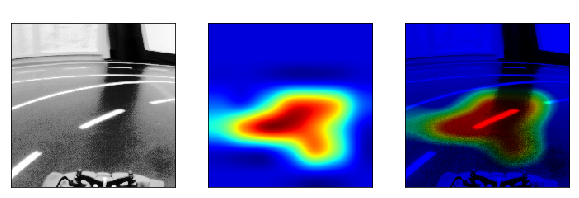
\includegraphics[width=\linewidth]{figures/right.png}	 
	%\caption{}
	%Quelle: \protect\citeI{Architecture-ALVINN}
	\label{img:right}
	\end{figure}
\end{frame}


\begin{frame}
\frametitle{Attention-Heatmap}
\framesubtitle{Kreuzung}

\begin{columns}[T]

\begin{column}[T]{2cm}
\quad \\
\quad \\
\textbf{Links} \\
\quad \\
\quad \\
\quad \\
\quad \\
\quad \\
\quad \\
\quad \\
\textbf{Rechts}	
\end{column}

\begin{column}[T]{8cm}
	\begin{figure}
	\centering
	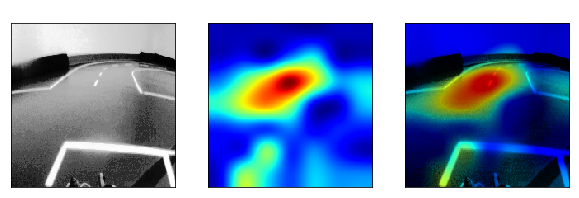
\includegraphics[width=\linewidth]{figures/kreuzungleft.png}	 
	%\caption{}
	%Quelle: \protect\citeI{Architecture-ALVINN}
	\label{img:kreuzungleft}
	\end{figure}

	\begin{figure}
	\centering
	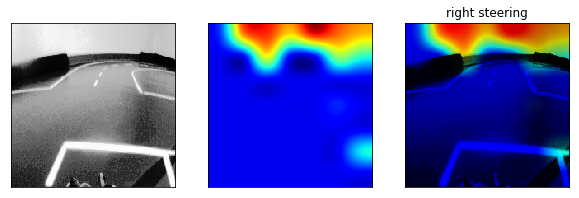
\includegraphics[width=\linewidth]{figures/kreuzungright.png}	 
	%\caption{}
	%Quelle: \protect\citeI{Architecture-ALVINN}
	\label{img:kreuzungright}
	\end{figure}
\end{column}

\end{columns}

\end{frame}

\section{Schluss}
\frame{\tableofcontents[currentsection]}

\begin{frame}
\frametitle{Bewertung}
Zielsetzung:\\
\begin{itemize}
\item{Steuerung mit neuronalem Netz entwickelt}
\item{Erprobung der Steuerung in Testfahrt}\\
$\xrightarrow{}$\textbf{Ziel erreicht}\\
\end{itemize}
\pause
Aber:\\
\begin{itemize}
\item{Begrenzte Testumgebung}\\
$\xrightarrow{}$Generalisierbarkeit unklar
\end{itemize}
\end{frame}

\begin{frame}
\frametitle{Ausblick}
Ansatzpunkte weiterer Fragestellungen:

\end{frame}

\begin{frame}
\frametitle{Quellen}

%\ref{img:chainrule} Quelle: https://becominghuman.ai/back-propagation-in-convolutional-neural-networks-intuition-and-code-714ef1c38199 \\

\end{frame}


\end{document}